\section*{14. Linear Regression}\label{linear-regression}

\textbf{Regression} is a method for studying the relationship between a
\textbf{response variable} \(Y\) and a \textbf{covariates} \(X\). The
covariate is also called a \textbf{predictor variable} or
\textbf{feature}. Later we will generalize and allow for more than one
covariate. The data are of the form

\[ (Y_{1}, X_{1}), \dots, (Y_{n}, X_{n}) \]

One way to summarize the relationship between \(X\) and \(Y\) is through
the \textbf{regression function}

\[ r(x) = \mathbb{E}(Y | X = x) = \int y f(y | x) dy \]

Most of this chapter is concerned with estimating the regression
function.

\subsection*{14.1 Simple Linear
Regression}\label{simple-linear-regression}

The simplest version of regression is when \(X_{i}\) is simple (a scalar,
not a vector) and \(r(x)\) is assumed to be linear:

\[r(x) = \beta_{0} + \beta_{1} x\]

This model is called the \textbf{simple linear regression model}. Let
\(\epsilon_{i} = Y_{i} - (\beta_{0} + \beta_{1} X_{i})\). Then:

\begin{align*}
\mathbb{E}(\epsilon_{i} | Y_{i}) &= \mathbb{E}(Y_{i} - (\beta_{0} + \beta_{1} X_{i}) | X_{i})\\
&= \mathbb{E}(Y_{i} | X_{i}) - (\beta_{0} + \beta_{1} X_{i})\\
&= r(X_{i}) - (\beta_{0} + \beta_{1} X_{i})\\
&= 0
\end{align*}

Let \(\sigma^{2}(x) = \mathbb{V}(\epsilon_{i} | X_{i} = x)\). We will make the
further simplifying assumption that \(\sigma^{2}(x) = \sigma^{2}\) does not
depend on \(x\).

\textbf{The Linear Regression Model}

\[Y_{i} = \beta_{0} + \beta_{1} X_{i} + \epsilon_{i}\]

where \(\mathbb{E}(\epsilon_{i} | X_{i}) = 0\) and
\(\mathbb{V}(\epsilon_{i} | X_{i}) = \sigma^{2}\).

The unknown models in the parameter are the intercept \(\beta_{0}\), the
slope \(\beta_{1}\) and the variance \(\sigma^{2}\). Let \(\hat{\beta_{0}}\)
and \(\hat{\beta_{1}}\) denote the estimates of \(\beta_{0}\) and
\(\beta_{1}\). The \textbf{fitted line} is defined to be

\[\hat{r}(x) = \hat{\beta}_{0} + \hat{\beta}_{1} x\]

The \textbf{predicted values} or \textbf{fitted values} are
\(\hat{Y}_{i} = \hat{r}(X_{i})\) and the \textbf{residuals} are defined to
be

\[\hat{\epsilon}_{i} = Y_{i} - \hat{Y}_{i} = Y_{i} - (\hat{\beta}_{0} + \hat{\beta}_{1} X_{i})\]

The \textbf{residual sum of squares} or RSS is defined by

\[ \text{RSS} = \sum_{i=1}^{n} \hat{\epsilon}_{i}^{2}\]

The quantity RSS measures how well the fitted line fits the data.

The \textbf{least squares estimates} are the values \(\hat{\beta}_{0}\)
and \(\hat{\beta}_{1}\) that minimize
\(\text{RSS} = \sum_{i=1}^{n} \hat{\epsilon}_{i}^{2}\).

\textbf{Theorem 14.4}. The least square estimates are given by

\begin{align*}
\hat{\beta}_{1} &= \frac{\sum_{i=1}^{n} (X_{i} - \overline{X}_{n}) (Y_{i} - \overline{Y}_{n})}{\sum_{i=1}^{n} (X_{i} - \overline{X}_{n})^{2}}\\
\hat{\beta}_{0} &= \overline{Y}_{n} - \hat{\beta}_{1} \overline{X}_{n}
\end{align*}

An unbiased estimate of \(\sigma^{2}\) is

\[
\hat{\sigma}^{2} = \left( \frac{1}{n - 2} \right) \sum_{i=1}^{n} \hat{\epsilon}_{i}^{2}
\]

\subsection*{14.2 Least Squares and Maximum
Likelihood}\label{least-squares-and-maximum-likelihood}

Suppose we add the assumption that
\(\epsilon_{i} | X_{i} \sim N(0, \sigma^{2})\), that is,

\(Y_{i} | X_{i} \sim N(\mu_{i}, \sigma_{i}^{2})\)

where \(\mu_{i} = \beta_{0} + \beta_{i} X_{i}\). The likelihood function is

\begin{align*}
\prod_{i=1}n f(X_{i}, Y_{i}) &= \prod_{i=1}^{n} f_X(X_{i}) f_{Y|X}(Y_{i} | X_{i})\\
&= \prod_{i=1}^{n} f_X(X_{i}) \times \prod_{i=1}^{n} f_{Y|X}(Y_{i} | X_{i}) \\
&= \mathcal{L}_{1} \times \mathcal{L}_{2}
\end{align*}

where \(\mathcal{L}_{1} = \prod_{i=1}^{n} f_X(X_{i})\) and
\(\mathcal{L}_{2} = \prod_{i=1}^{n} f_{Y|X}(Y_{i} | X_{i})\).

The term \(\mathcal{L}_{1}\) does not involve the parameters \(\beta_{0}\)
and \(\beta_{1}\). We shall focus on the second term \(\mathcal{L}_{2}\)
which is called the \textbf{conditional likelihood}, given by

\[\mathcal{L}_{2} \equiv \mathcal{L}(\beta_{0}, \beta_{1}, \sigma)
= \prod_{i=1}^{n} f_{Y|X}(Y_{i} | X_{i})
\propto \sigma^{-n} \exp \left\{ - \frac{1}{2 \sigma^{2}} \sum_{i} (Y_{i} - \mu_{i})^{2} \right\}
\]

The conditional log-likelihood is

\[\ell(\beta_{0}, \beta_{1}, \sigma) = -n \log \sigma - \frac{1}{2 \sigma^{2}} \sum_{i=1}^{n} \left(Y_{i} - (\beta_{0} + \beta_{1} X_{i}) \right)^{2}\]

To find the MLE of \((\beta_{0}, \beta_{1})\) we maximize the conditional
log likelihood. We can see from the equation above that this is the same
as minimizing the RSS. Therefore, we have shown the following:

\textbf{Theorem 14.7}. Under the assumption of Normality, the least
squares estimator is also the maximum likelihood estimator.

We can also maximize \(\ell(\beta_{0}, \beta_{1}, \sigma)\) over \(\sigma\)
yielding the MLE

\[ \hat{\sigma}^{2} = \frac{1}{n} \sum_{i=1}^{n} \hat{\epsilon}_{i}^{2} \]

This estimator is similar to, but not identical to, the unbiased
estimator. Common practice is to use the unbiased estimator.

\subsection*{14.3 Properties of the Least Squares
Estimators}\label{properties-of-the-least-squares-estimators}

\textbf{Theorem 14.8}. Let
\(\hat{\beta}^T = (\hat{\beta}_{0}, \hat{\beta}_{1})^T\) denote the least
squares estimators. Then,

\[
\mathbb{E}(\hat{\beta} | X^{n}) = \begin{pmatrix}\beta_{0} \\ \beta_{1} \end{pmatrix}
\]

\[
\mathbb{V}(\hat{\beta} | X^{n}) = \frac{\sigma^{2}}{n s_X^{2}} \begin{pmatrix} 
\frac{1}{n} \sum_{i=1}^{n} X_{i}^{2} & -\overline{X}_{n} \\
-\overline{X}_{n} & 1
\end{pmatrix}
\]

where \(s_X^{2} = n^{-1} \sum_{i=1}^{n} (X_{i} - \overline{X}_{n})^{2}\).

The estimated standard errors of \(\hat{\beta}_{0}\) and \(\hat{\beta}_{1}\)
are obtained by taking the square roots of the corresponding diagonal
terms of \(\mathbb{V}(\hat{\beta} | X^{n})\) and inserting the estimate
\(\hat{\sigma}\) for \(\sigma\). Thus,

\begin{align*}
\hat{\text{se}}(\hat{\beta}_{0}) &= \frac{\hat{\sigma}}{s_X \sqrt{n}} \sqrt{\frac{\sum_{i=1}^{n} X_{i}^{2}}{n}}\\
\hat{\text{se}}(\hat{\beta}_{1}) &= \frac{\hat{\sigma}}{s_X \sqrt{n}}
\end{align*}

We should write \(\hat{\text{se}}(\hat{\beta}_{0} | X^{n})\) and
\(\hat{\text{se}}(\hat{\beta}_{1} | X^{n})\) but we will use the shorter
notation \(\hat{\text{se}}(\hat{\beta}_{0})\) and
\(\hat{\text{se}}(\hat{\beta}_{1})\).

\textbf{Theorem 14.9}. Under appropriate conditions we have:

\begin{enumerate}[label={\arabic*.}]
\item
  (Consistency) \(\hat{\beta}_{0} \xrightarrow{\text{P}} \beta_{0}\) and
  \(\hat{\beta}_{1} \xrightarrow{\text{P}} \beta_{1}\)
\item
  (Asymptotic Normality):
\end{enumerate}

\[
\frac{\hat{\beta}_{0} - \beta_{0}}{\hat{se}(\hat{\beta}_{0})} \leadsto N(0, 1)
\quad \text{and} \quad
\frac{\hat{\beta}_{1} - \beta_{1}}{\hat{se}(\hat{\beta}_{1})} \leadsto N(0, 1)
\]

\begin{enumerate}[tightlist,label={\arabic*.},resume]
\item
  Approximate \(1 - \alpha\) confidence intervals for \(\beta_{0}\) and
  \(\beta_{1}\) are
\end{enumerate}

\[
\hat{\beta}_{0} \pm z_{\alpha/2} \hat{\text{se}}(\hat{\beta}_{0})
\quad \text{and} \quad
\hat{\beta}_{1} \pm z_{\alpha/2} \hat{\text{se}}(\hat{\beta}_{1})
\]

The Wald statistic for testing \(H_{0} : \beta_{1} = 0\) versus
\(H_{1}: \beta_{1} \neq 0\) is: reject \(H_{0}\) if \(W > z_{\alpha / 2}\)
where \(W = \hat{\beta}_{1} / \hat{\text{se}}(\hat{\beta}_{1})\).

\subsection*{14.4 Prediction}\label{prediction}

Suppose we have estimated a regression model
\(\hat{r}(x) = \hat{\beta}_{0} + \hat{\beta}_{1} x\) from data
\((X_{1}, Y_{1}), \dots, (X_{n}, Y_{n})\). We observe the value \(X_* = x\) of
the covariate for a new subject and we want to predict the outcome
\(Y_*\). An estimate of \(Y_*\) is

\[ \hat{Y}_* = \hat{\beta}_{0} + \hat{\beta}_{1} X_*\]

Using the formula for the variance of the sum of two random variables,

\[ \mathbb{V}(\hat{Y}_*) = \mathbb{V}(\hat{\beta}_{0} + \hat{\beta}_{1} x_*) = \mathbb{V}(\hat{\beta}_{0}) + x_* \mathbb{V}(\hat{\beta}_{1}) + 2 x_* \text{Cov}(\hat{\beta}_{0}, \hat{\beta}_{1}) \]

Theorem 14.8 gives the formulas for all terms in this equation. The
estimated standard error \(\hat{\text{se}}(\hat{Y}_*)\) is the square
root of this variance, with \(\hat{\sigma}^{2}\) in place of \(\sigma^{2}\).
However, \textbf{the confidence interval for \(\hat{Y}_*\) is not of the
usual form} \(\hat{Y}_* \pm z_{\alpha} \hat{\text{se}}(\hat{Y}_*)\). The
appendix explains why. The correct form is given in the following
Theorem. We can the interval a \textbf{prediction interval}.

\textbf{Theorem 14.11 (Prediction Interval)}. Let

\begin{align*}
\hat{\xi}_{n}^{2} &= \hat{\text{se}}^{2}(\hat{Y}_*) + \hat{\sigma}^{2} \\
&= \hat{\sigma}^{2} \left(\frac{\sum_{i=1}^{n} (X_{i} - X_*)^{2}}{n \sum_{i=1}^{n} (X_{i} - \overline{X})^{2}} + 1 \right)
\end{align*}

An approximate \(1 - \alpha\) prediction interval for \(Y_*\) is

\[ \hat{Y}_* \pm z_{\alpha/2} \xi_{n}\]

\subsection*{14.5 Multiple Regression}\label{multiple-regression}

Now suppose we have \(k\) covariates \(X_{1}, \dots, X_{k}\). The data are
of the form

\[(Y_{1}, X_{1}), \dots, (Y_{n}, X_{n})\]

where

\[ X_{i} = (X_{i1}, \dots, X_{ik}) \]

Here, \(X_{i}\) is the vector of \(k\) covariates for the \(i-\)th
observation. The linear regression model is

\[ Y_{i} = \sum_{i=1}^{k} \beta_{j} X_{ij} + \epsilon_{i} \]

for \(i = 1, \dots, n\) where
\(\mathbb{E}(\epsilon_{i} | X_{1i}, \dots, X_{ik}) = 0\). Usually we want
to include an intercept in the model which we can do by setting
\(X_{i1} = 1\) for \(i = 1, \dots, n\). At this point it will become
more convenient to express the model in matrix notation. The outcomes
will be denoted by

\[ Y = \begin{pmatrix}
Y_{1} \\
Y_{2} \\
\vdots \\
Y_{n}
\end{pmatrix}
\]

and the covariates will be denoted by

\[ X = \begin{pmatrix}
X_{11} & X_{12} & \cdots & X_{1k} \\
X_{21} & X_{22} & \cdots & X_{2k} \\
\vdots & \vdots & \ddots & \vdots \\
X_{n1} & X_{n2} & \cdots & X_{nk}
\end{pmatrix}
\]

Each row is one observation; the columns represent to the \(k\)
covariates. Thus, \(X\) is a \(n \times k\) matrix. Let

\[
\beta = \begin{pmatrix}
\beta_{1} \\
\vdots \\
\beta_{k}
\end{pmatrix}
\quad \text{and} \quad
\epsilon = \begin{pmatrix}
\epsilon_{1} \\
\vdots \\
\epsilon_{k}
\end{pmatrix}
\]

Then we can write the linear regression model as

\[ Y = X \beta + \epsilon \]

\textbf{Theorem 14.13}. Assuming that the \(k \times k\) matrix \(X^TX\)
is invertible, the least squares estimate is

\[ \hat{\beta} = (X^T X)^{-1} X^T Y \]

The estimated regression function is

\[ \hat{r}(x) = \sum_{j=1}^{k} \hat{\beta}_{j} x_{j}\]

The variance-covariance matrix of \(\hat{\beta}\) is

\[ \mathbb{V}(\hat{\beta} | X^{n}) = \sigma^{2} (X^T X)^{-1} \]

An unbiased estimate of \(\sigma^{2}\) is

\[ \hat{\sigma}^{2} = \left( \frac{1}{n - k} \right) \sum_{i=1}^{n} \hat{\epsilon}_{i}^{2} \]

where \(\hat{\epsilon} = X \hat{\beta} - Y\) is the vector of residuals.
An approximate \(1 - \alpha\) confidence interval for \(\beta_{j}\) is

\[ \hat{\beta}_{j} \pm z_{\alpha/2} \hat{\text{se}}(\hat{\beta}_{j}) \]

where \(\hat{\text{se}}^{2}(\hat{\beta}_{j})\) is the \(j\)-th diagonal
element of the matrix \(\hat{\sigma}^{2} (X^T X)^{-1}\).

\subsection*{14.6 Model Selection}\label{model-selection}

We may have data on many covariates but we may not want to include all
of them in the model. A smaller model with fewer covariates has two
advantages: it might give better predictions than a big model and it is
more parsimonious (simpler). Generally, as you add more variables to a
regression, the bias of the predictions decreases and the variance
increases. Too few covariates yields high bias; too many covariates
yields high variance. Good predictions result from achieving a good
balance between bias and variance.

In model selection there are two problems: assigning a score to each
model which measures, in some sense, how good the model is, and
searching through all models to find the model with the best score.

Let \(S \subset \{1, \dots, k\}\) and let
\(\mathcal{X}_S = \{ X_{j} : j \in S \}\) denote a subset of the
covariates. Let \(\beta_S\) denote the coefficients of the corresponding
set of covariates and let \(\hat{\beta}_S\) denote the least squares
estimate of \(\beta_S\). Let \(X_S\) denote the \(X\) matrix for this
subset of covariates, and let \(\hat{r}_S(x)\) to be the estimated
regression function. The predicted values from model \(S\) are denoted
by \(\hat{Y}_{i}(S) = \hat{r}_S(X_{i})\).

The \textbf{prediction risk} is defined to be

\[R(S) = \sum_{i=1}^{n} \mathbb{E} (\hat{Y}_{i}(S) - Y_{i}^*)^{2} \]

where \(Y_{i}^*\) denotes the value of the future observation of \(Y_{i}\)
at covariate value \(X_{i}\). Our goal is to choose \(S\) to make \(R(S)\)
small.

The \textbf{training error} is defined to be

\[\hat{R}_\text{tr}(S) = \sum_{i=1}^{n} (\hat{Y}_{i}(S) - Y_{i})^{2} \]

This estimate is very biased and under-estimates \(R(S)\).

\textbf{Theorem 14.15}. The training error is a downward biased estimate
of the prediction risk:

\[ \mathbb{E}(\hat{R}_\text{tr}(S)) < R(S) \]

In fact,

\[\text{bias}(\hat{R}_\text{tr}(S)) = \mathbb{E}(\hat{R}_\text{tr}(S)) - R(S) = -2 \sum_{i=1}^{n} \text{Cov}(\hat{Y}_{i}, Y_{i})\]

The reason for the bias is that the data is being used twice: to
estimate the parameters and to estimate the risk. When fitting a model
with many variables, the covariance \(\text{Cov}(\hat{Y_{i}}, Y_{i})\) will
be large and the bias of the training error gets worse.

In summary, the training error is a poor estimate of risk. Here are some
better estimates.

\textbf{Mallow's \(C_p\) statistic} is defined by

\[\hat{R}(S) = \hat{R}_\text{tr}(S) + 2 |S| \hat{\sigma}^{2}\]

where \(|S|\) denotes the number of terms in \(S\) and
\(\hat{\sigma}^{2}\) is the estimate of \(\sigma^{2}\) obtained from the
full model (with all covariates). Think of the \(C_p\) statistic as lack
of fit plus complexity penalty.

A related method for estimating risk is \textbf{AIC (Akaike Information
Criterion)}. The idea is to choose \(S\) to maximize

\[ \ell_S - |S|\]

where \(\ell_S\) is the log-likelihood of the model evaluated at the
MLE. In linear regression with Normal errors, maximizing AIC is
equivalent to minimizing Mallow's \(C_p\); see exercise 8.

\emph{Some texts use a slightly different definition of AIC which
involves multiplying this definition by 2 or -2. This has no effect on
which model is selected.}

Yet another method for estimating risk is \textbf{leave-one-out
cross-validation}. In this case, the risk estimator is

\[\hat{R}_\text{CV}(S) = \sum_{i=1}^{n} (Y_{i} - \hat{Y}_{(i)})^{2} \]

where \(\hat{Y}_{(i)}\) is the prediction for \(Y_{i}\) obtained by
fitting the model with \(Y_{i}\) omitted. It can be shown that

\[\hat{R}_\text{CV}(S) = \sum_{i=1}^{n} \left( \frac{Y_{i} - \hat{Y}_{i}(S)}{1 - U_{ii}(S)} \right)^{2} \]

where \(U_{i}i\) is the \(i\)-th diagonal element of the matrix

\[U(S) = X_S (X_S^T X_S)^{-1} X_S^T\]

Thus one need not actually drop each observation and re-fit the model.

A generalization is \textbf{k-fold cross-validation}. Here we divide the
data into \(k\) groups; often people take \(k = 10\). We omit one group
of data and fit the models on the remaining data. We use the fitted
model to predict the data in the group that was omitted. We then
estimate the risk by \(\sum_{i} (Y_{i} - \hat{Y}_{i})^{2}\) where the sum is
over the data points in the omitted group. This process is repeated for
each of the \(k\) groups and the resulting risk estimates are averaged.

For linear regression, Mallows \(C_p\) and cross-validation often yield
essentially the same results so one might as well use Mallow's method.
In some of the more complex problems we will discuss later,
cross-validation will be more useful.

Another scoring method is \textbf{BIC (Bayesian Information Criterion)}.
Here we choose a model to maximize

\[ \text{BIC}(S) = \text{RSS}(S) = 2 |S| \hat{\sigma}^{2} \]

The BIC score has a Bayesian interpretation. Let
\(\mathcal{S} = \{ S_{1}, \dots, S_m \}\) denote a set of models. Suppose
we assign the uniform prior \(\mathbb{P}(S_{j}) = 1 / m\) over the models.
Also assume we put a smooth prior on the parameters within each model.
It can be shown that the posterior probability for a model is
approximately

\[ \mathbb{P}(S_{j} | \text{data}) \approx \frac{e^{\text{BIC}(S_{j})}}{\sum_r e^{\text{BIC}(S_r)}}\]

so choosing the model with highest BIC is like choosing the model with
highest posterior probability.

The BIC score also has an information-theoretical interpretation in
terms of something called minimum description length.

The BIC score is identical to Mallows \(C_p\) except that it puts a more
severe penalty for complexity. It thus leads one to choose a smaller
model than the other methods.

If there are \(k\) covariates then there are \(2^{k}\) possible models. We
need to search through all of those models, assign a score to each one,
and choose the model with the best score. When \(k\) is large, this is
infeasible; in that case, we need to search over a subset of all the
models. Two common methods are \textbf{forward and backward stepwise
regression}.

In forward stepwise regression, we start with no covariates in the
model, and keep adding variables one at a time that lead to the best
score. In backward stepwise regression, we start with the biggest model
(all covariates) and drop one variable at a time.

\subsection*{14.7 The Lasso}\label{the-lasso}

This method, due to Tibshirani, is called the \textbf{Lasso}. Assume
that all covariates have been rescaled to have the same variance.
Consider estimating \(\beta = (\beta_{1}, \dots, \beta_{k})\) by minimizing
the loss function

\[ \sum_{i=1}^{n} (Y_{i} - \hat{Y}_{i})^{2} + \lambda \sum_{j=1}^{k} | \beta_{j} |\]

where \(\lambda > 0\). The idea is to minimize the sums of squares but
there is a penalty that gets large if any \(\beta_{j}\) gets large. It can
be shown that some of the \(\beta_{j}\)Here is will be 0. We interpret this as
having the \(j\)-th covariate omitted from the model; thus we are doing
estimation and model selection simultaneously.

We need to choose a value of \(\lambda\). We can do this by estimating
the prediction risk \(R(\lambda)\) as a function of \(\lambda\) and
choosing to minimize it. For example, we can estimate the risk using
leave-one-out cross-validation

\subsection*{14.8 Technical Appendix}

The prediction interval is of a different form than other confidence
intervals we have seen -- the quantity of interest \(Y_*\) is equal to a
parameter \(\theta\) plus a random variable.

We can fix this by defining:

\[ \xi_{n}^{2} = \mathbb{V}(\hat{Y}_*) + \sigma^{2} = \left[\frac{\sum_{i} (x_{i} - x_*)^{2}}{n \sum_{i} (x_{i} - \overline{x})^{2}} + 1\right] \sigma^{2}\]

In practice, we substitute \(\hat{\sigma}\) for \(\sigma\) and we denote
the resulting quantity by \(\hat{\xi}_{n}\). Now,

\begin{align*}
\mathbb{P}(\hat{Y}_* - z_{\alpha/2} \hat{\xi}_{n} < Y_* < \hat{Y}_* + z_{\alpha/2} \hat{\xi}_{n}) &=
\mathbb{P}\left(-z_{\alpha/2} < \frac{\hat{Y}_* - Y_*}{\hat{\xi}_{n}} < z_{\alpha/2} \right)\\
&= \mathbb{P}\left(-z_{\alpha/2} < \frac{\hat{\theta} - \theta - \epsilon}{\hat{\xi}_{n}} < z_{\alpha/2} \right) \\
&\approx \mathbb{P}\left(-z_{\alpha/2} < \frac{N(0, s^{2} + \sigma^{2})}{\hat{\xi}_{n}} < z_{\alpha/2} \right)  \\
&\approx \mathbb{P}\left(-z_{\alpha/2} < \frac{N(0, s^{2} + \sigma^{2})}{\xi_{n}} < z_{\alpha/2} \right)  \\
&= \mathbb{P}(-z_{\alpha/2} < N(0, 1) < z_{\alpha/2}) \\
&= 1 - \alpha
\end{align*}

\subsection*{14.9 Exercises}

\textbf{Exercise 14.9.1}. Prove Theorem 14.4:

The least square estimates are given by

\begin{align*}
\hat{\beta}_{1} &= \frac{\sum_{i=1}^{n} (X_{i} - \overline{X}_{n}) (Y_{i} - \overline{Y}_{n})}{\sum_{i=1}^{n} (X_{i} - \overline{X}_{n})^{2}}\\
\hat{\beta}_{0} &= \overline{Y}_{n} - \hat{\beta}_{1} \overline{X}_{n}
\end{align*}

An unbiased estimate of \(\sigma^{2}\) is

\[
\hat{\sigma}^{2} = \left( \frac{1}{n - 2} \right) \sum_{i=1}^{n} \hat{\epsilon}_{i}^{2}
\]

\textbf{Solution}. We can obtain the estimates \(\hat{\beta}_{0}\) and
\(\hat{\beta}_{1}\) by minimizing the RSS -- by taking the partial
derivatives with respect to \(\beta_{0}\) and \(\beta_{1}\):

\[\text{RSS} = \sum_{i} \hat{\epsilon}_{i}^{2} = \sum_{i} (Y_{i} - (\beta_{0} + \beta_{1} X_{i}))^{2}\]

Derivating RSS on \(\beta_{0}\):

\[\frac{d}{d \beta_{0}}\text{RSS} = \sum_{i} \frac{d}{d \beta_{0}} (Y_{i} - (\beta_{0} + \beta_{1} X_{i}))^{2}
= \sum_{i} 2 (\beta_{0} - (Y_{i} - \beta_{1} X_{i}))\]

Making this derivative equal to 0 at \(\hat{\beta}_{0}\),
\(\hat{\beta}_{1}\) gives:

\begin{align*}
0 &= \sum_{i} 2 (\hat{\beta}_{0} - (Y_{i} - \hat{\beta}_{1} X_{i}))\\
n \hat{\beta}_{0} &= n \sum_{i} Yi - \hat{\beta}_{1} n \sum_{i} X_{i}\\
\hat{\beta}_{0} &= \overline{Y}_{n} - \hat{\beta}_{1} \overline{X}_{n}
\end{align*}

Replacing \(\overline{Y}_{n} - \beta_{1} \overline{X}_{n}\) for \(\beta_{0}\)
and derivating on \(\beta_{1}\):

\[\frac{d}{d \beta_{1}}\text{RSS} = \sum_{i} \frac{d}{d \beta_{1}} (Y_{i} - (\beta_{0} + \beta_{1} X_{i}))^{2}
\sum_{i} \frac{d}{d \beta_{1}} (Y_{i} - \overline{Y}_{n} - \beta_{1} (X_{i} - \overline{X}_{n})))^{2}
= \sum_{i} -2 (X_{i} - \overline{X}_{n}) (Y_{i} - \overline{Y}_{n} - \beta_{1} (X_{i} - \overline{X}_{n})))\]

Making this derivative equal to 0 at \(\hat{\beta}_{1}\) gives:

\begin{align*}
0 &= \sum_{i} (X_{i} - \overline{X}_{n}) (Y_{i} - \overline{Y}_{n} - \beta_{1} (X_{i} - \overline{X}_{n}))) \\
0 &= \hat{\beta}_{1} \sum_{i} (\overline{X}_{n} - X_{i})^{2} + \sum_{i} (\overline{X}_{n} - X_{i})(Y_{i} - \overline{Y}_{n}) \\
\hat{\beta}_{1} &= \frac{\sum_{i} (X_{i} - \overline{X}_{n})(Y_{i} - \overline{Y}_{n})}{\sum_{i} (X_{i} - \overline{X}_{n})^{2}}
\end{align*}

For the unbiased estimate,  adapt a more general proof from Greene
(2003), restricted to \(k = 2\) dimensions, where the first dimension is
set to all ones to represent the intercept, and the second dimension
represents the one-dimensional covariates \(X_{i}\).

The vector of least square residuals is

\[ \hat{\epsilon} = \begin{pmatrix}
\hat{\epsilon}_{1} \\
\hat{\epsilon}_{2} \\
\vdots \\
\hat{\epsilon}_{n}
\end{pmatrix} = \begin{pmatrix}
Y_{1} - (\hat{\beta}_{0} \cdot 1 + \hat{\beta}_{1} X_{1}) \\
Y_{2} - (\hat{\beta}_{0} \cdot 1 + \hat{\beta}_{1} X_{2}) \\
\vdots \\
Y_{n} - (\hat{\beta}_{0} \cdot 1 + \hat{\beta}_{1} X_{n})
\end{pmatrix} = 
y - X \hat{\beta}
\]

where \[
y = \begin{pmatrix}
Y_{1} \\
Y_{2} \\
\vdots \\
Y_{n}
\end{pmatrix}
, \quad
X = \begin{pmatrix}
1 & X_{1} \\
1 & X_{2} \\
\vdots & \vdots \\
1 & X_{n}
\end{pmatrix},
\quad \text{and} \quad
\hat{\beta} = \begin{pmatrix}
\hat{\beta}_{0} \\
\hat{\beta}_{1}
\end{pmatrix}
\]

The least squares solution can be written as:

\[\hat{\beta} = (X^T X)^{-1} X^T y\]

Replacing it on the definition of \(\hat{\epsilon}\), we get

\[ \hat{\epsilon} = y - X (X^T X)^{-1} X^T y = (I - X (X^T X)^{-1} X^T) y = M y\]

where \(M = I - X (X^T X)^{-1} X^T\) is known as the \textbf{residual
maker} matrix.

Note that \(M\) is symmetric, that is, \(M^T = M\):

\begin{align*}
M^T &= (I - X (X^T X)^{-1} X^T)^T  \\
&= I^T - (X (X^T X)^{-1} X^T)^T \\
&= I - (X^T)^T ((X^T X)^{-1})^T X^T \\
&= I - X ((X^{-1}(X^T)^{-1})^T X^T \\
&= I -  X (X^T X)^{-1} X^T \\
&= M
\end{align*}

Note also that \(M\) is idempotent, that is, \(M^{2} = M\):

\begin{align*}
M^{2} &= (I - X (X^T X)^{-1} X^T) (I - X (X^T X)^{-1} X^T) \\
&= I - X (X^T X)^{-1} X^T - X (X^T X)^{-1} X^T + X \left( (X^T X)^{-1} X^T X \right) (X^T X)^{-1} X^T \\
&= I - X (X^T X)^{-1} X^T - X (X^T X)^{-1} X^T + X (X^T X)^{-1} X^T \\
&= I - X (X^T X)^{-1} X^T \\
&= M
\end{align*}

Now, we have that \(MX = 0\), as running least squares on a regression
where the covariates match the target variables should yield a model
that just copies the covariate over, where all residuals are zero
(\(\beta_{0} = 0\) and \(\beta_{1} = 1\)). So:

\[\hat{\epsilon} = M y = M( X \beta + \epsilon) = M\epsilon\]

where \(\epsilon = Y - X\beta\) are the population residuals.

We can then write an estimator for \(\sigma^{2}\):

\[ \hat{\epsilon}^T \hat{\epsilon} = \epsilon^T M^T M \epsilon = \epsilon^T M^{2} \epsilon = \epsilon^T M \epsilon\]

Taking the expectation with respect to the data \(X\) on both sides,

\[\mathbb{E}(\hat{\epsilon}^T \hat{\epsilon} | X) = \mathbb{E}(\epsilon^T M \epsilon | X)\]

But \(\epsilon^T M \epsilon\) is a scalar (\(1 \times 1\) matrix), so it
is equal to its trace -- and we can use the cyclic permutation property
of the trace:

\[ \mathbb{E}(\epsilon^T M \epsilon | X) = \mathbb{E}(\text{tr}(\epsilon^T M \epsilon) | X) = \mathbb{E}(\text{tr}(M \epsilon \epsilon^T) | X)\]

Since \(M\) is a function of \(X\), we can take it out of the
expectation:

\[\mathbb{E}(\text{tr}(M \epsilon \epsilon^T) | X) = \text{tr}(\mathbb{E}(M \epsilon \epsilon^T | X))
= \text{tr}(M \mathbb{E}(\epsilon \epsilon^T | X))
= \text{tr}(M \sigma^{2} I_{1})
= \sigma^{2} \text{tr}(M)
\]

Finally, we can compute the trace of \(M\):

\begin{align*}
\text{tr}(M) &= \text{tr}(I_{n} - X(X^T X)^{-1}X^T)\\
&= \text{tr}(I_{n}) - \text{tr}(X(X^T X)^{-1}X^T) \\
&= \text{tr}(I_{n}) - \text{tr}((X^T X)^{-1}X^T X) \\
&= \text{tr}(I_{n}) - \text{tr}(I_{k})  \\
&= n - k
\end{align*}

Therefore, the unbiased estimator is

\[\hat{\sigma}^{2} = \frac{\hat{\epsilon}^T \hat{\epsilon}}{n - k}\]

or, for our case where \(k = 2\),

\[\hat{\sigma}^{2} = \left( \frac{1}{n - 2} \right) \sum_{i=1}^{n} \hat{\epsilon}_{i}^{2}\]

Reference: Greene, William H. Econometric analysis. Pearson Education
India, 2003. Chapter 4, pages 61-62.

\textbf{Exercise 14.9.2}. Prove the formulas for the standard errors in
Theorem 14.8. You should regard the \(X_{i}\)Here is as fixed constants.

\[
\mathbb{E}(\hat{\beta} | X^{n}) = \begin{pmatrix}\beta_{0} \\ \beta_{1} \end{pmatrix}
\quad \text{and} \quad
\mathbb{V}(\hat{\beta} | X^{n}) = \frac{\sigma^{2}}{n s_X^{2}} \begin{pmatrix} 
\frac{1}{n} \sum_{i=1}^{n} X_{i}^{2} & -\overline{X}_{n} \\
-\overline{X}_{n} & 1
\end{pmatrix}
\]

\[s_X^{2} = n^{-1} \sum_{i=1}^{n} (X_{i} - \overline{X}_{n})^{2}\]

\[
\hat{\text{se}}(\hat{\beta}_{0}) = \frac{\hat{\sigma}}{s_X \sqrt{n}} \sqrt{\frac{\sum_{i=1}^{n} X_{i}^{2}}{n}}
\quad \text{and} \quad
\hat{\text{se}}(\hat{\beta}_{1}) = \frac{\hat{\sigma}}{s_X \sqrt{n}}
\]

\textbf{Solution}.

The formulas follow immediately by performing the suggested replacement
on the diagonal elements of \(\mathbb{V}(\hat{\beta} | X^{n})\) from
Theorem 14.8. From the diagonals, replacing \(\hat{\sigma}\) for
\(\sigma\):

\[
\hat{\text{se}}(\hat{\beta}_{0})^{2} = \frac{\hat{\sigma}^{2}}{n s_X^{2}} \frac{\sum_{i=1}^{n} X_{i}^{2}}{n}
\quad \text{and} \quad
\hat{\text{se}}(\hat{\beta}_{1})^{2} = \frac{\hat{\sigma}^{2}}{n s_X^{2}} \cdot 1\]

Results follow by taking the square root.

We will also prove the variance matrix result itself, following from the
notation and proof used on exercise 14.9.1 (again, adapting from
Greene):

\[
\hat{\beta} = (X^T X)^{-1}X^T y = (X^T X)^{-1}X^T (X \beta + \epsilon) = \beta + (X^T X)^{-1}X^T \epsilon
\]

Taking the variance conditional on \(X\),

\begin{align*}
\mathbb{V}(\hat{\beta} | X) &= \mathbb{V}(\hat{\beta} - \beta | X) \\
&= \mathbb{E}((\hat{\beta} - \beta)(\hat{\beta} - \beta)^T | X)  \\
&= \mathbb{E}((X^T X)^{-1}X^T \epsilon\epsilon^T X(X^T X)^{-1} | X) \\
&= (X^T X)^{-1}X^T \mathbb{E}(\epsilon\epsilon^T | X) X(X^T X)^{-1} \\
&= (X^T X)^{-1}X^T \sigma^{2} I X(X^T X)^{-1} \\
&= \sigma^{2} (X^T X)^{-1} 
\end{align*}

But we have:

\[ X^T X = \begin{pmatrix}
1 & 1 & \cdots & 1 \\
X_{1} & X_{2} & \cdots & X_{n}
\end{pmatrix} \begin{pmatrix}
1 & X_{1} \\
1 & X_{2} \\
\vdots & \vdots \\
1 & X_{n}
\end{pmatrix} = 
n \begin{pmatrix}
1 & \overline{X}_{n} \\
\overline{X}_{n} & \frac{1}{n}\sum_{i=1}^{n} X_{i}^{2}
\end{pmatrix}
\]

so we can verify its inverse is

\[(X^T X)^{-1} = \frac{1}{n s_X^{2}} \begin{pmatrix}
\frac{1}{n} \sum_{i=1}^{n} X_{i}^{2} & - \overline{X}_{n} \\
-\overline{X}_{n} & 1
\end{pmatrix}\]

and so the result follows.

Reference: Greene, William H. Econometric analysis. Pearson Education
India, 2003. Chapter 4, page 59.

\textbf{Exercise 14.9.3}. Consider the \textbf{regression through the
origin} model:

\[Y_{i} = \beta X_{i} + \epsilon\]

Find the least squares estimate for \(\beta\). Find the standard error
of the estimate. Find conditions that guarantee that the estimate is
consistent.

\textbf{Solution}. Once more adopting notation from the solution of
14.9.1, let

\[ y = \begin{pmatrix} Y_{1} \\ \vdots \\ Y_{n} \end{pmatrix},
\quad
X = \begin{pmatrix} X_{1} \\ \vdots \\ X_{n} \end{pmatrix}\]

and \(\beta\) is a scalar (or a \(1 \times 1\) matrix).

The least squares estimate is, again,

\[\hat{\beta} = (X^T X)^{-1} X^T y\]

which simplifies in this one-dimensional case to:

\[\hat{\beta} = \frac{\sum_{i=1}^{n} X_{i} Y_{i}}{\sum_{i=1}^{n} X_{i}^{2}}\]

The unbiased estimator for \(\sigma^{2}\) is, with \(k = 1\),

\[\hat{\sigma}^{2} = \frac{1}{n - 1} \sum_{i=1}^{n} \hat{\epsilon}_{i}^{2}\]

and the variance of \(\hat{\beta}\) conditional of \(X\) is:

\[\mathbb{V}(\hat{\beta} | X) = \sigma^{2} (X^T X)^{-1} = \frac{\sigma^{2}}{\sum_{i=1}^{n} X_{i}^{2}}\]

so the standard error of the estimate is

\[\hat{\text{se}}(\hat{\beta}) = \frac{\hat{\sigma}}{\sqrt{\sum_{i=1}^{n} X_{i}^{2}}}\]

These, of course, make the assumption that \(X^T X\) is invertible --
that is, that the sum of squares of the \(X_{i}\) variables is greater
than 0. This is only not the case when all covariates are 0, in which
case the value of our estimator \(\hat{\beta}\) would be irrelevant to
determining the prediction outcome -- the system would be undetermined.

Finally, note that \(\hat{\beta}\) is also the MLE in the parameter
space for regression through the origin. As each measurement error
\(\epsilon_{i} = Y_{i} - \beta X_{i}\) is drawn from a normal distribution
\(N(0, \sigma^{2})\), the log-likelihood for a given parameter \(\beta\)
is

\[\ell_{n}(\beta) = -\frac{n}{2} \log \sigma^{2} - \frac{1}{2 \sigma^{2}} \sum_{i=1}^{n} (Y_{i} - \beta X_{i})^{2} + C\]

and so maximizing it is equivalent to minimizing
\(\sum_{i=1}^{n} (Y_{i} - \beta X_{i})^{2}\), which is what the least squares
procedure does.

Since the MLE is consistent, the least squares estimate is also
consistent.

\textbf{Exercise 14.9.4}. Prove equation (14.24).

\[ \text{bias}(\hat{R}_\text{tr}(S)) = \mathbb{E}(\hat{R}_\text{tr}(S)) - R(S) = -2 \sum_{i} \text{Cov}(\hat{Y}_{i}, Y_{i}) \]

\textbf{Solution}.

The bias is:

\begin{align*}
\mathbb{E}(\hat{R}_\text{tr}(S)) - R(S) &= \mathbb{E}\left[\sum_{i} (\hat{Y}_{i}- Y_{i})^{2} \right] - \mathbb{E} \left[ \sum_{i} (\hat{Y}_{i} - Y_{i}^*)^{2} \right] \\
&= \sum_{i} \left( \mathbb{E} \left[\hat{Y}_{i}^{2} \right] - 2 \mathbb{E} \left[\hat{Y}_{i} Y_{i} \right] + \mathbb{E}\left[Y_{i}^{2} \right] - \mathbb{E} \left[\hat{Y}_{i}^{2} \right] + 2 \mathbb{E} \left[\hat{Y}_{i} Y_{i}^* \right] - \mathbb{E}\left[{Y_{i}^*}^{2} \right] \right)
\end{align*}

The random variables \(Y_{i} = \beta X_{i} + \epsilon_\text{train}\) and
\(Y_{i}^* = \beta X_{i} + \epsilon_\text{pred}\) are independent, as the
errors during training and predition are independent, and the covariates
\(X_{i}\) and true parameter \(\beta\) are constant. Since they are
independent,
\(\mathbb{E}[Y_{i} Y_{i}^*] = \mathbb{E}[Y_{i}] \mathbb{E}[Y_{i}^*]\).

We also have
\(\mathbb{E} [ {Y_{i}^*}^{2} ] = \mathbb{V}[Y_{i}^*] + \mathbb{E}[Y_{i}^*]^{2} = \mathbb{V}[\epsilon_\text{pred}] + \mathbb{E}[X \beta]^{2} = \mathbb{V}[\epsilon_\text{train}] + \mathbb{E}[Y_{i}]^{2} = \mathbb{E} [Y_{i}^{2}]\).

Replacing both of those in the expression of bias above, we get the
result:

\begin{align*}
\mathbb{E}(\hat{R}_\text{tr}(S)) - R(S) &= 
-2 \sum_{i} \left( \mathbb{E}[Y_{i} \hat{Y}_{i}] - \mathbb{E}[Y_{i}] \mathbb{E}[\hat{Y}_{i}] \right) \\
&= -2 \sum_{i} \text{Cov}(\hat{Y}_{i}, Y_{i})
\end{align*}

\textbf{Exercise 14.9.5}. In the simple linear regression model,
construct a Wald test for \(H_{0} : \beta_{1} = 17 \beta_{0}\) versus
\(H_{1} : \beta_{1} \neq 17 \beta_{0}\).

\textbf{Solution}. Let \(\delta = \beta_{1} - 17 \beta_{0}\). The MLE is
\(\hat{\delta} = \hat{\beta}_{1} - 17 \hat{\beta}_{0}\), with estimated
standard error \(\hat{\text{se}}(\hat{\delta})\), where

\[\hat{\text{se}}(\hat{\delta})^{2} = \hat{\text{se}}(\hat{\beta}_{1} - 17 \hat{\beta}_{0})^{2} = \hat{\text{se}}(\hat{\beta}_{1})^{2} + 17^{2} \hat{\text{se}}(\hat{\beta}_{0})^{2} \]

and the estimates for the parameter standard deviations are

\[
\hat{\text{se}}(\hat{\beta}_{0}) = \frac{\hat{\sigma}}{s_X \sqrt{n}} \sqrt{\frac{\sum_{i=1}^{n} X_{i}^{2}}{n}}
\quad \text{and} \quad
\hat{\text{se}}(\hat{\beta}_{1}) = \frac{\hat{\sigma}}{s_X \sqrt{n}}
\]

The Wald test then checks if \(|W| < z_{\alpha / 2}\), where

\[W = \frac{\hat{\delta} - 0}{\hat{\text{se}}(\hat{\delta})} 
= \frac{\hat{\beta}_{1} - 17 \hat{\beta}_{0}}{\sqrt{\hat{\text{se}}(\hat{\beta}_{1})^{2} + 17^{2} \hat{\text{se}}(\hat{\beta}_{0})^{2}}}\]

\textbf{Exercise 14.9.6}. Get the passenger car mileage data from

\url{http://lib.stat.cmu.edu/DASL/Datafiles/carmpgdat.html}

\textbf{(a)} Fit a simple linear regression model to predict MPG (miles
per gallon) from HP (horsepower). Summarize your analysis including a
plot of the data with the fitted line.

\textbf{(b)} Repeat the analysis but use log(MPG) as the response.
Compare the analysis.

\textbf{Solution}.

We would ordinarily use a library to do linear regression, but given
this chapter is specifically on linear regression formulas, consider all
of the calculations on matrix algebra ``by hand'' instead -- and compare
the results with statsmodels OLS.

\begin{python}
import numpy as np
import pandas as pd
from scipy.stats import t
import statsmodels.api as sm
import matplotlib.pyplot as plt

# Provided link is dead.  Data was found elsewhere online.
data = pd.read_csv('data/carmileage.csv')
\end{python}

\begin{python}
def get_regression(X, Y):
    X = X.copy()
    
    # Create new column with all 1s for intercept at start
    X.insert(0, 'const', 1)
    
    # Least squares solution
    beta_hat = (np.linalg.inv(X.T @ X) @ X.T @ Y).to_{n}umpy()

    # Predicted solutions
    Y_pred = X @ beta_hat

    # Prediction errors
    epsilon_hat = Y_pred - Y

    # Error on training data
    training_error = epsilon_hat.T @ epsilon_hat
    
    # Estimated error variance
    sigma2_hat = (training_error / (Y.shape[0] - X.shape[1]))

    # Parameter estimated standard errors
    se_beta_hat = np.sqrt(sigma2_hat * np.diag(np.linalg.inv(X.T @ X))).T

    # t statistic for estimated parameters being non-zero
    t_values = beta_hat.reshape(-1) / se_beta_hat

    # p-values for estimated parameters being non-zero
    p_values = 2 * (1 - t.cdf(np.abs(t_values), X.shape[0] - 1))
    
    return pd.DataFrame({
        'coef': beta_hat.reshape(-1),
        'std err': se_beta_hat.reshape(-1),
        't': t_values.reshape(-1),
        'P > |t|': p_values.reshape(-1) 
        }, index=X.columns)
\end{python}


\textbf{(a)}

\begin{python}
Y = data['MPG']
X = data[['HP']]
\end{python}

\begin{python}
# Using manually coded solution
get_regression(X, Y)
\end{python}

\begin{console}
	coef	std err	t	P > |t|
const	50.066078	1.569487	31.899650	0.0
HP	-0.139023	0.012069	-11.519295	0.0
\end{console}

\begin{python}
# Using statsmodels
results = sm.OLS(Y, sm.add_constant(X)).fit()
print(results.summary())
\end{python}

\begin{console}
                            OLS Regression Results
==============================================================================
Dep. Variable:                    MPG   R-squared:                       0.624
Model:                            OLS   Adj. R-squared:                  0.619
Method:                 Least Squares   F-statistic:                     132.7
Date:                Sun, 15 Mar 2020   Prob (F-statistic):           1.15e-18
Time:                        17:06:26   Log-Likelihood:                -264.61
No. Observations:                  82   AIC:                             533.2
Df Residuals:                      80   BIC:                             538.0
Df Model:                           1
Covariance Type:            nonrobust
==============================================================================
                 coef    std err          t      P>|t|      [0.025      0.975]
------------------------------------------------------------------------------
const         50.0661      1.569     31.900      0.000      46.943      53.189
HP            -0.1390      0.012    -11.519      0.000      -0.163      -0.115
==============================================================================
Omnibus:                       22.759   Durbin-Watson:                   0.721
Prob(Omnibus):                  0.000   Jarque-Bera (JB):               31.329
Skew:                           1.246   Prob(JB):                     1.57e-07
Kurtosis:                       4.722   Cond. No.                         299.
==============================================================================

Warnings:
[1] Standard Errors assume that the covariance matrix of the errors is correctly
specified.
\end{console}

\begin{python}
# Plotting results

fig, ax = plt.subplots(figsize=(12, 8))
fig = sm.graphics.plot_fit(results, 1, ax=ax)
plt.show()
\end{python}

\begin{figure}[H]
\centering
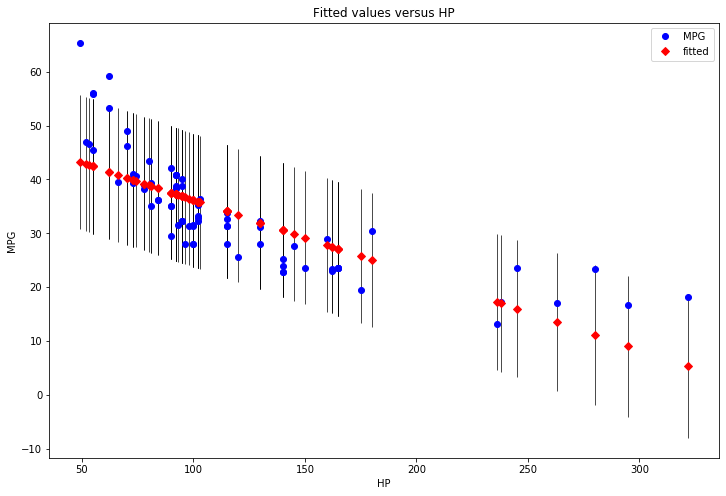
\includegraphics{Figure-14-01}
\end{figure}

\textbf{(b)}

\begin{python}
# Exactly the same exercise, but fit on a different response variable

Y = np.log(data['MPG']).rename('log MPG')
X = data[['HP']]
\end{python}

\begin{python}
# Using manually coded solution
get_regression(X, Y)
\end{python}

\begin{console}
	coef	std err	t	P > |t|
const	4.013229	0.040124	100.021194	0.0
HP	-0.004589	0.000309	-14.873129	0.0
\end{console}

\begin{python}
# Using statsmodels
results = sm.OLS(Y, sm.add_constant(X)).fit()
print(results.summary())
\end{python}

\begin{console}
                            OLS Regression Results
==============================================================================
Dep. Variable:                log MPG   R-squared:                       0.734
Model:                            OLS   Adj. R-squared:                  0.731
Method:                 Least Squares   F-statistic:                     221.2
Date:                Sun, 15 Mar 2020   Prob (F-statistic):           9.62e-25
Time:                        17:06:26   Log-Likelihood:                 36.047
No. Observations:                  82   AIC:                            -68.09
Df Residuals:                      80   BIC:                            -63.28
Df Model:                           1
Covariance Type:            nonrobust
==============================================================================
                 coef    std err          t      P>|t|      [0.025      0.975]
------------------------------------------------------------------------------
const          4.0132      0.040    100.021      0.000       3.933       4.093
HP            -0.0046      0.000    -14.873      0.000      -0.005      -0.004
==============================================================================
Omnibus:                        4.454   Durbin-Watson:                   1.026
Prob(Omnibus):                  0.108   Jarque-Bera (JB):                3.827
Skew:                           0.516   Prob(JB):                        0.148
Kurtosis:                       3.236   Cond. No.                         299.
==============================================================================

Warnings:
[1] Standard Errors assume that the covariance matrix of the errors is correctly
specified.
\end{console}

\begin{python}
# Plotting results

fig, ax = plt.subplots(figsize=(12, 8))
fig = sm.graphics.plot_fit(results, 1, ax=ax)
plt.show()
\end{python}

\begin{figure}[H]
\centering
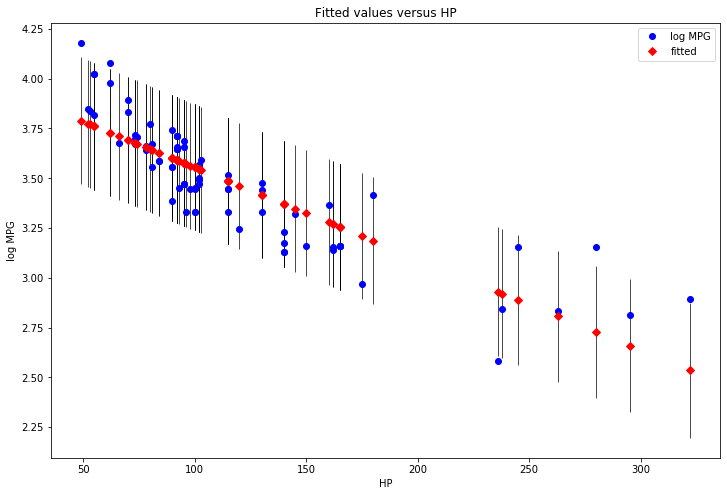
\includegraphics{Figure-14-02}
\end{figure}

\textbf{Exercise 14.9.7}. Get the passenger car mileage data from

\url{http://lib.stat.cmu.edu/DASL/Datafiles/carmpgdat.html}

\textbf{(a)} Fit a multiple linear regression model to predict MPG
(miles per gallon) from HP (horsepower). Summarize your analysis
including a plot of the data with the fitted line.

\textbf{(b)} Use Mallow's \(C_p\) to select a best sub-model. To search
through all models try (i) all possible models, (ii) forward stepwise,
(iii) backward stepwise. Summarize your findings.

\textbf{(c)} Repeat (b) but use BIC. Compare the results.

\textbf{(d)} Now use Lasso and compare the results.

\textbf{Solution}.

The exercise wording is unclear -- if we specify that HP is the only
covariate, the multiple linear regression and the simple linear
regression are the same, and (a) is like the previous exercise.

We will elect to use VOL, HP, SP and WT as the covariates, and MPG as
the response variable.

\textbf{(a)}

\begin{python}
# Use full model

features = ['HP', 'SP', 'WT', 'VOL']

Y = data['MPG']
X = data[features]
\end{python}

\begin{python}
# Using manually coded solution
get_regression(X, Y)
\end{python}

\begin{console}
             coef    std err         t       P > |t|
const  192.437753  23.531613  8.177839  3.351097e-12
HP       0.392212   0.081412  4.817602  6.671547e-06
SP      -1.294818   0.244773 -5.289864  1.019119e-06
WT      -1.859804   0.213363 -8.716617  2.888800e-13
VOL     -0.015645   0.022825 -0.685425  4.950327e-01
\end{console}
        
\begin{python}
# Using statsmodels
results = sm.OLS(Y, sm.add_constant(X)).fit()
print(results.summary())
\end{python}

\begin{console}
                            OLS Regression Results
==============================================================================
Dep. Variable:                    MPG   R-squared:                       0.873
Model:                            OLS   Adj. R-squared:                  0.867
Method:                 Least Squares   F-statistic:                     132.7
Date:                Sun, 15 Mar 2020   Prob (F-statistic):           9.98e-34
Time:                        17:06:27   Log-Likelihood:                -220.00
No. Observations:                  82   AIC:                             450.0
Df Residuals:                      77   BIC:                             462.0
Df Model:                           4
Covariance Type:            nonrobust
==============================================================================
                 coef    std err          t      P>|t|      [0.025      0.975]
------------------------------------------------------------------------------
const        192.4378     23.532      8.178      0.000     145.580     239.295
HP             0.3922      0.081      4.818      0.000       0.230       0.554
SP            -1.2948      0.245     -5.290      0.000      -1.782      -0.807
WT            -1.8598      0.213     -8.717      0.000      -2.285      -1.435
VOL           -0.0156      0.023     -0.685      0.495      -0.061       0.030
==============================================================================
Omnibus:                       14.205   Durbin-Watson:                   1.148
Prob(Omnibus):                  0.001   Jarque-Bera (JB):               18.605
Skew:                           0.784   Prob(JB):                     9.12e-05
Kurtosis:                       4.729   Cond. No.                     1.16e+04
==============================================================================

Warnings:
[1] Standard Errors assume that the covariance matrix of the errors is correctly
specified.
[2] The condition number is large, 1.16e+04. This might indicate that there are
strong multicollinearity or other numerical problems.
\end{console}

\begin{python}
# Plotting results

fig, ax = plt.subplots(figsize=(12, 8))
fig = sm.graphics.plot_fit(results, 1, ax=ax)
ax.set_ylabel("MPG")
ax.set_xlabel("HP")
ax.set_title("Linear Regression")
plt.show()
\end{python}

\begin{figure}[H]
\centering
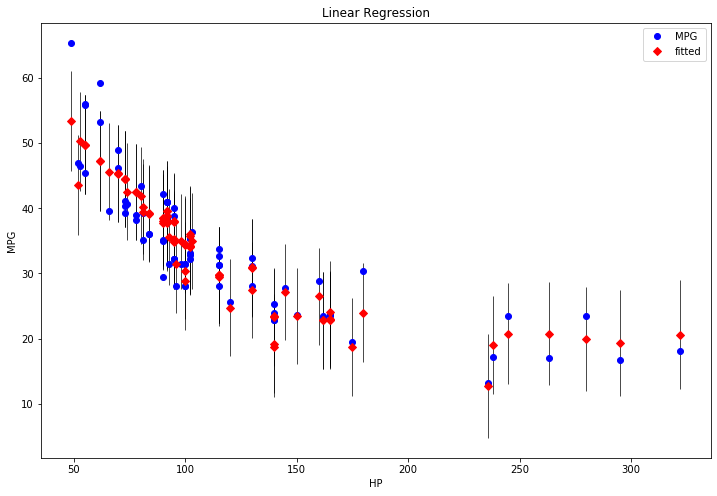
\includegraphics{Figure-14-03}
\end{figure}

\textbf{(b)}

First,  create helper functions to calculate the model variance and
Mallow's \(C_p\):

\begin{python}
def get_model_variance(X, Y):
    X = X.copy()
    
    # Create new column with all 1s for intercept at start
    X.insert(0, 'const', 1)
    
    # Least squares solution
    beta_hat = (np.linalg.inv(X.T @ X) @ X.T @ Y).to_{n}umpy()

    # Predicted solutions
    Y_pred = X @ beta_hat

    # Prediction errors
    epsilon_hat = Y_pred - Y

    # Error on training data
    training_error = epsilon_hat.T @ epsilon_hat
    
    # Estimated error variance
    return (training_error / (Y.shape[0] - X.shape[1]))
    

def get_mallow_cp(X, Y, S, full_model_variance):
    if len(S) > 0:
        X = X[list(S)].copy()
        # Create new column with all 1s for intercept at start
        X.insert(0, 'const', 1)
    else:
        X = pd.DataFrame({'const': np.ones_like(Y)})
    
    # Least squares solution
    beta_hat = (np.linalg.inv(X.T @ X) @ X.T @ Y).to_{n}umpy()

    # Predicted solutions
    Y_pred = X @ beta_hat

    # Prediction errors
    epsilon_hat = Y_pred - Y

    # Error on training data
    partial_training_error = epsilon_hat.T @ epsilon_hat
    
    # Increase size of S by to account for constant covariate
    return partial_training_error + 2 * (len(S) + 1) * full_model_variance
\end{python}

Next,  calculate and save the full model variance \textbf{once},
sine it is used for every candidate model -- and use it to define our
custom score function.

\begin{python}
full_model_variance = get_model_variance(X, Y)

def score_mallow_cp(S):
    return get_mallow_cp(X, Y, S, full_model_variance)
\end{python}

Finally, consider the submodel search.

First approach is an explicit search through all features:

\begin{python}
from itertools import chain, combinations

def powerset(iterable):
    "powerset([1,2,3]) --> () (1,) (2,) (3,) (1,2) (1,3) (2,3) (1,2,3)"
    s = list(iterable)
    return chain.from_{i}terable(combinations(s, r) for r in range(len(s)+1))
\end{python}

\begin{python}
# Iterate through the powerset and calculate the score for each value
results = [(S, score_mallow_cp(S)) for S in powerset(features)]
    
# Format as dataframe for ease of presentation
results = pd.DataFrame(results, columns=['S', 'score'])
\end{python}

\begin{python}
results
\end{python}

\begin{console}
                    S        score
0                  ()  8134.147794
1               (HP,)  3102.805578
2               (SP,)  4318.234609
3               (WT,)  1519.372094
4              (VOL,)  7059.223052
5            (HP, SP)  2436.578842
6            (HP, WT)  1510.677511
7           (HP, VOL)  2354.823180
8            (SP, WT)  1463.076513
9           (SP, VOL)  3056.598857
10          (WT, VOL)  1542.174631
11       (HP, SP, WT)  1140.390871
12      (HP, SP, VOL)  2147.886521
13      (HP, WT, VOL)  1507.484328
14      (SP, WT, VOL)  1443.795004
15  (HP, SP, WT, VOL)  1160.807643
\end{console}
       
\begin{python}
results[results.score == results.score.min()]
\end{python}

\begin{console}
               S        score
11  (HP, SP, WT)  1140.390871
\end{console}

This approach recommends the features HP, SP, and WT.

Next, consider forward stepwise feature selection:

\begin{python}
current_subset = []
current_score = score_mallow_cp(current_subset)

while len(current_subset) < len(features):
    best_score, best_subset = current_score, current_subset
    updated = False
    for f in features:
        if f not in current_subset:
            candidate_subset = current_subset + [f]
            candidate_score = score_mallow_cp(candidate_subset)
            if candidate_score < best_score:
                best_score, best_subset = candidate_score, candidate_subset
                updated = True              
    if not updated:
        break
        
    current_score, current_subset = best_score, best_subset
    
pd.DataFrame([[tuple(current_subset), current_score]], columns=['S', 'score'])
\end{python}

\begin{console}
              S        score
0  (WT, SP, HP)  1140.390871
\end{console}

This approach also recommends selecting these 3 features (order is
irrelevant): WT, SP, HP

Finally, apply backward stepwise feature selection:

\begin{python}
current_subset = features
current_score = score_mallow_cp(current_subset)

while len(current_subset) > 0:
    best_score, best_subset = current_score, current_subset
    updated = False
    for f in features:
        if f in current_subset:
            candidate_subset = [a for a in current_subset if a != f]
            candidate_score = score_mallow_cp(candidate_subset)
            if candidate_score < best_score:
                best_score, best_subset = candidate_score, candidate_subset
                updated = True              
    if not updated:
        break
        
    current_score, current_subset = best_score, best_subset
    
pd.DataFrame([[tuple(current_subset), current_score]], columns=['S', 'score'])
\end{python}

\begin{console}
              S        score
0  (HP, SP, WT)  1140.390871
\end{console}

This approach also recommends selecting the same 3 features.

\textbf{(c)} This is analogous to (b), using the new scoring function.

Note that the book's definition of BIC is:

\[ \text{BIC}(S) = \text{RSS}(S) + 2 |S| \hat{\sigma}^{2} \]

while other sources apply a log to this quantity and scale it by the
number of observations \(n\), e.g.

\[ \text{BIC} = n \log \left( \text{RSS} / n \right) + |S| \log n \]

We will use the later definition for this exercise.

\begin{python}
def get_bic(X, Y, S):
    if len(S) > 0:
        X = X[list(S)].copy()
        # Create new column with all 1s for intercept at start
        X.insert(0, 'const', 1)
    else:
        X = pd.DataFrame({'const': np.ones_like(Y)})
    
    # Least squares solution
    beta_hat = (np.linalg.inv(X.T @ X) @ X.T @ Y).to_{n}umpy()

    # Predicted solutions
    Y_pred = X @ beta_hat

    # Prediction errors
    epsilon_hat = Y_pred - Y

    # Error on training data
    rss = epsilon_hat.T @ epsilon_hat
    
    n = Y.shape[0]
    k = X.shape[1]
    
    return n * np.log(rss / n) + k * np.log(n)

def score_bic(S):
    return get_bic(X, Y, S)
\end{python}

Full search:

\begin{python}
# Iterate through the powerset and calculate the score for each value
results = [(S, score_bic(S)) for S in powerset(features)]
    
# Format as dataframe for ease of presentation
results = pd.DataFrame(results, columns=['S', 'score'])
\end{python}

\begin{python}
results
\end{python}

\begin{console}
                    S       score
0                  ()  381.100039
1               (HP,)  305.324815
2               (SP,)  332.832040
3               (WT,)  245.266568
4              (VOL,)  373.531556
5            (HP, SP)  288.594470
6            (HP, WT)  247.670065
7           (HP, VOL)  285.699095
8            (SP, WT)  244.895261
9           (SP, VOL)  307.747647
10          (WT, VOL)  249.455822
11       (HP, SP, WT)  225.425717
12      (HP, SP, VOL)  281.219751
13      (HP, WT, VOL)  250.346085
14      (SP, WT, VOL)  246.530268
15  (HP, SP, WT, VOL)  229.333642
\end{console}

\begin{python}

\end{python}

\begin{console}
               S       score
11  (HP, SP, WT)  225.425717
\end{console}

Forward stepwise:

\begin{python}
current_subset = []
current_score = score_bic(current_subset)

while len(current_subset) < len(features):
    best_score, best_subset = current_score, current_subset
    updated = False
    for f in features:
        if f not in current_subset:
            candidate_subset = current_subset + [f]
            candidate_score = score_bic(candidate_subset)
            if candidate_score < best_score:
                best_score, best_subset = candidate_score, candidate_subset
                updated = True              
    if not updated:
        break
        
    current_score, current_subset = best_score, best_subset
    
pd.DataFrame([[tuple(current_subset), current_score]], columns=['S', 'score'])
\end{python}

\begin{console}
              S       score
0  (WT, SP, HP)  225.425717
\end{console}

Backward stepwise:

\begin{python}
current_subset = features
current_score = score_bic(current_subset)

while len(current_subset) > 0:
    best_score, best_subset = current_score, current_subset
    updated = False
    for f in features:
        if f in current_subset:
            candidate_subset = [a for a in current_subset if a != f]
            candidate_score = score_bic(candidate_subset)
            if candidate_score < best_score:
                best_score, best_subset = candidate_score, candidate_subset
                updated = True              
    if not updated:
        break
        
    current_score, current_subset = best_score, best_subset
    
pd.DataFrame([[tuple(current_subset), current_score]], columns=['S', 'score'])
\end{python}

\begin{console}
              S       score
0  (HP, SP, WT)  225.425717
\end{console}

All approaches recommend the same feature selection as the previous
method -- select the 3 features HP, SP, and WT.

\textbf{(d)} To use Lasso, we will need to minimize the L1 loss function
for an arbitrary penalty parameter \(\lambda\):

\[ \sum_{i=1}^{n} (Y_{i} - \hat{Y}_{i})^{2} + \lambda \sum_{j=1}^{k} | \beta_{j} | \]

Since we are including a penalty parameter that affects both estimation
and model selection, we will need to calculate this loss function on
some test data distinct from the training data -- the recommended
approach being to use leave-one-out cross validation.

\begin{python}
from scipy.optimize import minimize

# Lasso loss function
def lasso_loss(Y, Y_pred, beta, l1_penalty):
    error = Y - Y_pred
    return error.T @ error + l1_penalty * sum(abs(beta))

# Regularized fit
def fit_regularized(X, Y, l1_penalty):
    def loss_function(beta):
        return lasso_loss(Y, X @ beta, beta, l1_penalty)
    
    # Use the solution without penalties as an initial guess
    beta_{i}nitial_guess = (np.linalg.inv(X.T @ X) @ X.T @ Y).to_{n}umpy()
    return minimize(loss_function, beta_{i}nitial_guess, method = 'Powell',
                    options={'xtol': 1e-8, 'disp': False, 'maxiter': 10000 }) 

# Leave-one-out cross-validation
def leave_one_out_cv_risk(X, Y, fitting_function):
    n = X.shape[1]
    total_risk = 0
    for i in range(n):
        XX = pd.concat([X.iloc[:i], X.iloc[i + 1:]])
        YY = pd.concat([Y.iloc[:i], Y.iloc[i + 1:]])
        beta = fitting_function(XX, YY).x
        validation_error = Y.iloc[i] - X.iloc[i] @ beta
        total_risk += validation_error * validation_error
    return total_risk / n

# Optimize over penalty parameter with best cross-validation risk
def optimize_l1_penalty(X, Y):
    def loss_function(l1_penalty_signed):
        # Ensure l1_penalty >= 0
        l1_penalty = abs(l1_penalty_signed)
        return leave_one_out_cv_risk(X, Y, lambda xx, yy: fit_regularized(xx, yy, l1_penalty))
    
    l1_penalty_{i}nitial_guess = 0.0
    return minimize(loss_function, l1_penalty_{i}nitial_guess, method = 'Powell',
                   options={'xtol': 1e-8, 'disp': True, 'maxiter': 10000 })
\end{python}

\begin{python}
# Create a new dimension with constants, so the regressions have an intercept
X_c = X.copy()
X_c.insert(0, 'const', 1)
\end{python}

\begin{python}
# Optimize cross validation risk over penalties
best_penalty_res = optimize_l1_penalty(X_c, Y)
selected_l1_penalty = abs(best_penalty_res.x)

print("Selected penalty: ", selected_l1_penalty)
\end{python}

\begin{console}
Optimization terminated successfully.
         Current function value: 61.554007
         Iterations: 1
         Function evaluations: 45
Selected penalty:  4.965056196086726e-07
\end{console}

\begin{python}
# Re-fit with selected penalty over the whole dataset
selected_fit = fit_regularized(X_c, Y, selected_l1_penalty)
beta = selected_fit.x
pd.DataFrame(beta.reshape(-1, 1), index=X_c.columns, columns=['coef'])
\end{python}

\begin{console}
             coef
const  192.437753
HP       0.392212
SP      -1.294818
WT      -1.859804
VOL     -0.015645
\end{console}

The best leave-one-out cross validation for the Lasso procedure is
achieved (according to our optimizer) at \(\lambda \approx\) 0, where
all covariants have a non-zero coefficient (i.e.~\(\beta_{i} \neq 0\) for
all \(i\)).

In other words, Lasso with leave-one-out cross validation selects the
full model.

\textbf{Exercise 14.9.8}. Assume that the errors are Normal. Show that
the model with highest AIC is the model with lowest Mallows \(C_p\)
statistic.

Mallows' \(C_p\):

\[\hat{R}(S) = \hat{R}_\text{tr}(S) + 2 |S| \hat{\sigma}^{2}\]

AIC:

\[  \text{AIC} = \ell_S - |S|\]

\textbf{Solution}.

For the given definition, note that
\(-2 \text{AIC} \hat{\sigma}^{2} = -2 \ell_S \hat{\sigma}^{2} + 2|S| \hat{\sigma}^{2} = \hat{R}_\text{tr}(S) + 2 |S| \hat{\sigma}^{2} = \hat{R}(S)\),
given the log likelihood of a Normal model -- so maximizing AIC is
equivalent to minimizing Mallows \(C_p\).

Note that a more general result holds: rather than assuming the errors
are Normal, one can assume that the distributions are part of a
spherically symmetric family, i.e., modifying the distributions under an
orthogonal transformation (and potentially removing invariance). See:
Boisbunon, Aurélie, et al.~``AIC, Cp and estimators of loss for
elliptically symmetric distributions.'' arXiv preprint arXiv:1308.2766
(2013).

\textbf{Exercise 14.9.9}. In this question we will take a closer look at the AIC method. Let \(X_{1}, \dots, X_{n}\) be iid observations. Consider two models \(\mathcal{M}_{0}\) and \(\mathcal{M}_{1}\). Under \(\mathcal{M}_{0}\) the data are assumed to be \(N(0, 1)\) while under \(M_{1}\) the data are assumed to be \(N(\theta, 1)\) for some unknown \(\theta \in \mathbb{R}\):

\begin{align*}
\mathcal{M}_{0} : X_{1}, \dots, X_{n} &\sim N(0, 1) \\
\mathcal{M}_{1} : X_{1}, \dots, X_{n} &\sim N(\theta, 1), \; \theta \in \mathbb{R}
\end{align*}

This is just another way of viewing the hypothesis testing problem: \(H_{0}: \theta = 0\) versus \(H_{1}: \theta \neq 0\). Let \(\ell_{n}(\theta)\) be the log-likelihood function. The AIC score for a model is the log-likelihood at the MLE minus the number of parameters. (Some people multiply this score by 2 but that is irrelevant). Thus, the AIC score for \(\mathcal{M}_{0}\) is \(\text{AIC}_{0} = \ell_{n}(0)\) and the AIC score for \(\mathcal{M}_{1}\) is \(\text{AIC}_{1} = \ell_{n}(\hat{\theta}) - 1\). Suppose we choose the model with highest AIC score. Let \(J_{n}\) denote the selected model:

\[
J_{n} = 
\begin{cases}
0 & \text{if } \text{AIC}_{0} > \text{AIC}_{1} \\
1 & \text{if } \text{AIC}_{1} > \text{AIC}_{0}
\end{cases}
\]

\textbf{(a)} Suppose that \(\mathcal{M}_{0}\) is the true model, i.e.~\(\theta = 0\). Find

\[ \lim_{n \rightarrow \infty} \mathbb{P}(J_{n} = 0) \]

Now compute \(\lim_{n \rightarrow \infty} \mathbb{P}(J_{n} = 0)\) when \(\theta \neq 0\).

\textbf{(b)} The fact that \(\lim_{n \rightarrow \infty} \mathbb{P}(J_{n} = 0) \neq 1\) when \(\theta = 0\) is why some people say that AIC ``overfits''. But this is not quite true as we shall now see. Let \(\phi_\theta(x)\) denote a Normal density function with mean \(\theta\) and variance 1. Define

\[ 
\hat{f}_{n}(x) = 
\begin{cases}
\phi_{0}(x) & \text{if } J_{n} = 0 \\
\phi_{\overline{\theta}}(x) & \text{if } J_{n} = 1
\end{cases}
\]

If \(\theta = 0\), show that
\(D(\phi_{0}, \hat{f}_{n}) \xrightarrow{\text{P}} 0\) as
\(n \rightarrow \infty\) where
\[ 
D(f, g) = \int f(x) \log \left( \frac{f(x)}{g(x)} \right) dx 
\]

is the Kullback-Leibler distance. Show that
\(D(\phi_\theta, \hat{f}_{n}) \xrightarrow{\text{P}} 0\) if
\(\theta \neq 0\). Hence, AIC consistently estimates the true density
even if it ``overshoots'' the correct model.

REMARK: If you are feeling ambitious, repeat the analysis for BIC which
is the log-likelihood minus \((p / 2) \log n\) where \(p\) is the number
of parameters and \(n\) is the sample size.

\textbf{Solution}.

\textbf{(a)} Note that the log-likelihood of the distribution
\(N(\mu, \sigma^{2})\) is:

\begin{align*}
\ell_{n}(\mu, \sigma^{2}) &= \log \prod_{i=1}^{n} f(X_{i} | \mu, \sigma^{2}) \\
&= \sum_{i=1}^{n} \log f(X_{i} | \mu, \sigma^{2}) \\
&= - \frac{n}{2} \log 2\pi - \frac{n}{2} \log \sigma^{2} - \frac{1}{2\sigma^{2}} \sum_{i=1}^{n} (X_{i} - \mu)^{2}
\end{align*}

Then, we have:

\begin{align*}
\mathbb{P}(J_{n} = 0) &= \mathbb{P}(\text{AIC}_{0} > \text{AIC}_{1}) \\
&= \mathbb{P}(\ell_{n}(0) > \ell_{n}(\hat{\theta}) - 1) \\
&= \mathbb{P} \left(-\frac{n}{2} \log 2\pi - 0 - \frac{1}{2} \sum_{i=1}^{n} (X_{i} - 0)^{2} > -\frac{n}{2} \log 2\pi - 0 - \frac{1}{2} \sum_{i=1}^{n} (X_{i} - \hat{\theta})^{2} - 1 \right) \\
&= \mathbb{P}\left( -\frac{1}{2} \sum_{i=1}^{n} X_{i}^{2} > -\frac{1}{2} \sum_{i=1}^{n} (X_{i} - \hat{\theta})^{2} - 1\right) \\
&= \mathbb{P}\left( \sum_{i=1}^{n} \left((X_{i} - \hat{\theta})^{2} - X_{i}^{2} \right) > -2 \right) \\
&= \mathbb{P}\left( n \hat{\theta}^{2} - 2 \hat{\theta} \sum_{i=1}^{n} X_{i} > -2 \right) \\
&= \mathbb{P}\left( n \overline{X}_{n}^{2} - 2 \overline{X}_{n} n \overline{X}_{n} > -2\right) \\
&= \mathbb{P}\left( -n \overline{X}_{n}^{2} > -2 \right) \\
&= \mathbb{P}\left(-\sqrt{\frac{2}{n}} < \overline{X}_{n} < \sqrt{\frac{2}{n}} \right)
\end{align*}

But \(X_{i} \sim N(\theta, 1)\), so
\(n \overline{X}_{n} = \sum_{i} X_{i} \sim N(n\theta, n)\) and
\(\overline{X}_{n} \sim N(\theta, 1/n)\). Then:

\begin{align*}
\mathbb{P}(J_{n} = 0) &= \mathbb{P}\left(-\sqrt{\frac{2}{n}} < \overline{X}_{n} < \sqrt{\frac{2}{n}} \right) \\
&= \mathbb{P}\left(\frac{-\sqrt{\frac{2}{n}} - \theta}{\sqrt{1/n}} < \frac{\overline{X}_{n} - \theta}{\sqrt{1/n}} < \frac{\sqrt{\frac{2}{n}} - \theta}{\sqrt{1/n}} \right) \\
&= \mathbb{P}\left(-\sqrt{2} - \sqrt{n}\theta < Z < \sqrt{2} - \sqrt{n}\theta \right) \\
&= \Phi(\sqrt{2} - \sqrt{n}\theta) - \Phi(-\sqrt{2} - \sqrt{n}\theta)
\end{align*}

where \(\Phi\) is the CDF of the standard normal distribution
\(N(0, 1)\).

When \(\theta = 0\),

\[\mathbb{P}(J_{n} = 0) = \Phi(\sqrt{2}) - \Phi(-\sqrt{2}) \approx 0.8427 \neq 0\]

When \(\theta \neq 0\),

\[\lim_{n \rightarrow \infty} \mathbb{P}(J_{n} = 0) = \lim_{n \rightarrow \infty}\Phi(\sqrt{2} - \sqrt{n}\theta) - \Phi(-\sqrt{2} - \sqrt{n}\theta) = \lim_{n \rightarrow \infty}\Phi(\sqrt{n}\theta) - \lim_{n \rightarrow \infty}\Phi(-\sqrt{n}\theta) = 0\]

\textbf{(b)} We have:

\[ D(\phi_\theta, \hat{f}_{n}) = \int \phi_\theta(x) \log \left(\frac{\phi_\theta(x)}{\hat{f}_{n}(x)} \right) dx = \int \left[\phi_\theta(x) \log \phi_\theta(x) - \phi_\theta(x) \log \hat{f}_{n}(x) \right] dx \]

But \(\lim_{n \rightarrow \infty} \hat{f}_{n}(x) = \phi_\theta(x)\), so
the integrand goes to 0 at each x, and so
\(D(\phi_\theta, \hat{f}_{n}) \xrightarrow{\text{P}} 0\).

\textbf{REMARK: I am feeling ambitious.} Let \(K_{n}\) denote the selected
model:

\[ K_{n} = \begin{cases}
0 & \text{if } \text{BIC}_{0} > \text{BIC}_{1} \\
1 & \text{if } \text{BIC}_{1} > \text{BIC}_{0}
\end{cases}\]

where

\[
\text{BIC}_{0} = \ell_{n}(0) \\
\text{BIC}_{1} = \ell_{n}(\hat{\theta}) - \frac{1}{2} \log n
\]

So,

\begin{align*}
\mathbb{P}(K_{n} = 0) &= \mathbb{P}(\text{BIC}_{0} > \text{BIC}_{1}) \\
&= \mathbb{P}\left(\ell_{n}(0) > \ell_{n}(\hat{\theta}) - \frac{1}{2} \log n \right) \\
&= \mathbb{P} \left(-\frac{n}{2} \log 2\pi - 0 - \frac{1}{2} \sum_{i=1}^{n} (X_{i} - 0)^{2} > -\frac{n}{2} \log 2\pi - 0 - \frac{1}{2} \sum_{i=1}^{n} (X_{i} - \hat{\theta})^{2} - \frac{1}{2} \log n \right) \\
&= \mathbb{P}\left( -\frac{1}{2} \sum_{i=1}^{n} X_{i}^{2} > -\frac{1}{2} \sum_{i=1}^{n} (X_{i} - \hat{\theta})^{2} - \frac{1}{2} \log n\right) \\
&= \mathbb{P}\left( \sum_{i=1}^{n} \left((X_{i} - \hat{\theta})^{2} - X_{i}^{2} \right) > -\log n \right) \\
&= \mathbb{P}\left( n \hat{\theta}^{2} - 2 \hat{\theta} \sum_{i=1}^{n} X_{i} > -\log n \right) \\
&= \mathbb{P}\left( n \overline{X}_{n}^{2} - 2 \overline{X}_{n} n \overline{X}_{n} > -\log n\right) \\
&= \mathbb{P}\left( -n \overline{X}_{n}^{2} > -\log n \right) \\
&= \mathbb{P}\left(-\sqrt{\frac{\log n}{n}} < \overline{X}_{n} < \sqrt{\frac{\log n}{n}} \right) \\
&= \mathbb{P}\left(\frac{-\sqrt{\frac{\log n}{n}} - \theta}{\sqrt{1/n}} < \frac{\overline{X}_{n} - \theta}{\sqrt{1/n}} < \frac{\sqrt{\frac{\log n}{n}} - \theta}{\sqrt{1/n}} \right) \\ 
&=  \mathbb{P}\left(-\sqrt{\log n} - \sqrt{n}\theta < Z < \sqrt{\log n} - \sqrt{n}\theta \right) \\
&= \Phi(\sqrt{\log n} - \sqrt{n}\theta) - \Phi(-\sqrt{\log n} - \sqrt{n}\theta)
\end{align*}

As \(O(\sqrt{log n}) < O(\sqrt{n})\), we get the result:

\[ \lim_{n \rightarrow \infty} \mathbb{P}(K_{n} = 0) = \begin{cases}
1 & \text{if } \theta = 0 \\
0 & \text{if } \theta \neq 0
\end{cases}\]

Also, if we define:

\[
\hat{g}_{n}(x) = 
\begin{cases}
\phi_{0}(x) & \text{if } K_{n} = 0 \\
\phi_{\overline{\theta}}(x) & \text{if } K_{n} = 1
\end{cases}
\]

then, again,

\[ D(\phi_\theta, \hat{g}_{n}) = \int \phi_\theta(x) \log \left(\frac{\phi_\theta(x)}{\hat{g}_{n}(x)} \right) dx = \int \left[\phi_\theta(x) \log \phi_\theta(x) - \phi_\theta(x) \log \hat{g}_{n}(x) \right] dx \]

But \(\lim_{n \rightarrow \infty} \hat{g}_{n}(x) = \phi_\theta(x)\), so
the integrand goes to 0 at each x, and so
\(D(\phi_\theta, \hat{g}_{n}) \xrightarrow{\text{P}} 0\).
